% Intro

\begin{frame}[c]
  \frametitle{Une double problématique}

La modélisation d'un système est la première étape vers sa compréhension

\begin{center}
  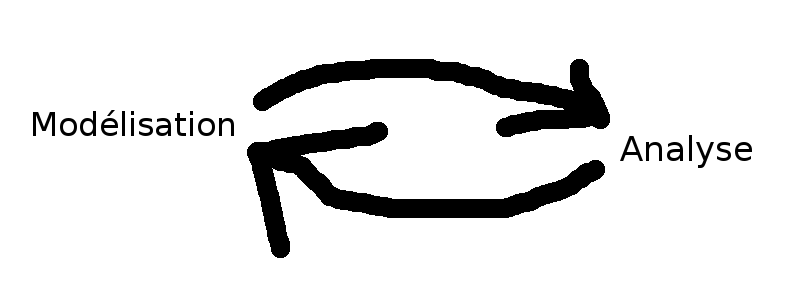
\includegraphics[width=.4\textwidth]{figs/modelanalyse.png}
\end{center}

L'analyse recherchée impacte les choix de modélisation
\begin{itemize}
  \item Les outils de modélisation doivent être adaptés aux propriétés observées
\end{itemize}

\medskip
Les choix de modélisation impactent les résultats de l'analyse
\begin{itemize}
  \item Un modèle trop grossier donne peu d'informations
  \item Un modèle de grande taille augmente le temps d'analyse
\end{itemize}

\medskip
\begin{center}
\tval{Les étapes de modélisation et d'analyse d'un système sont indissociables}
\end{center}

\end{frame}



\begin{frame}[c]
\frametitle{Plan}

\todo{LE PLAN}

État de l'art de la modélisation
\begin{itemize}
  \item Modélisations discrètes asynchrones
  \item Réseaux discrets et modèle de Thomas
  \item Frappes de Processus standards
\end{itemize}

Enrichissement des Frappes de Processus
\begin{itemize}
  \item Priorités
  \item Arcs neutralisants
  \item Actions plurielles
\end{itemize}

Analyse des Frappes de Processus
\begin{itemize}
  \item Correction des sortes coopératives
  \item Analyse statique pour l'atteignabilité
  \item Équivalences avec d'autres formalismes
\end{itemize}

\end{frame}
